\section{Using ENVISIoN's GUI}
\label{sec:newGUI}
ENVISIoN is equipped with a graphical user interface to simplify the usage of ENVISIoN. The newest version, as of 2021, of the graphical user interface is written in Python instead of JavaScript and HTML as the previous versions were. 

\subsection{Start-up}
When the user starts the application through the computer terminal (see chapter 5), a window opens for Ubuntu, see figure \ref{fig:newGUI}. The window has a column of boxes with empty datasets to the left, where the user can choose to load in different VASP-datasets och HDF5-files. The user can then choose an Empty Dataset box, and choose a VASP-directory or an already parsed HDF5-file to load. If a VASP-directroty has been selected the user can then parse the selected folder by pressing the "Parse Selected Folder" button. When a directory is chosen, and the dataset is parsed, the user can then choose the desired visualization. If a HDF5-file has been selected the files contents can be loaded into a dataset by pressing the "Load selected file in to dataset" button. After this the the user can start the visualizations in the same way as for the VASP-directory. Note that the system will only allow the user to choose visualizations which are possible given the chosen dataset. 

\begin{figure}[H]
    \centering
    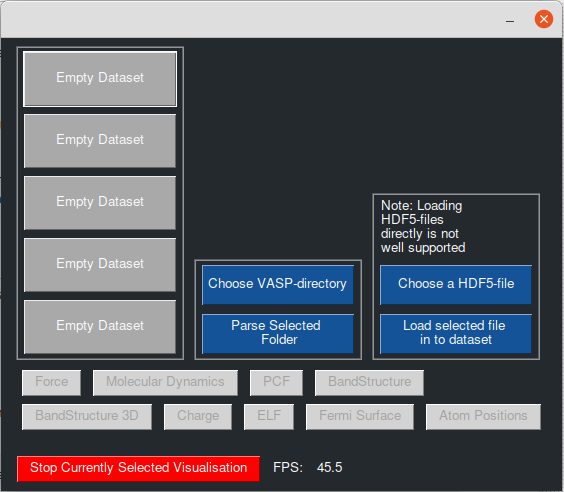
\includegraphics[scale = 0.56]{Images/newGUI.png}
    \caption{ENVISIoN GUI startup on Ubuntu.}
    \label{fig:newGUI}
\end{figure}

\subsection{Choose VASP-directory}
After choosing a Empty Dataset to load the VASP file, by pressing one of the "Empty Dataset" buttons, see figure \ref{fig:newGUI}, the user has to choose a VASP-directory to load. \newline \newline 

\subsubsection{Load a VASP file}
Figure \ref{fig:newGUI_resources} shows a folder with VASP-directories available for parsing. The user chooses which VASP-directory to parse, and then clicks "OK". Note that it is not sufficient to only highlight which folder the user wants to parse. The user has to double click the folder, and then click "OK", as shown in figure \ref{fig:newGUI_VASPdir}.

\begin{figure}[H]
    \centering
    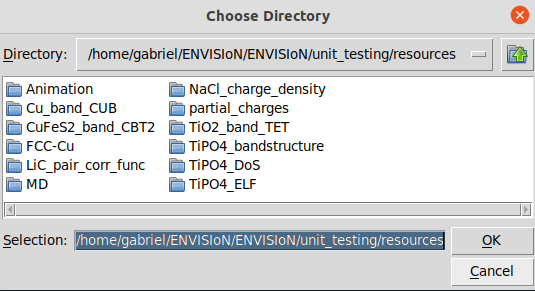
\includegraphics[scale = 0.56]{Images/newGUI_resources.png}
    \caption{VASP-directories available for parsing.}
    \label{fig:newGUI_resources}
\end{figure}

\begin{figure}[H]
    \centering
    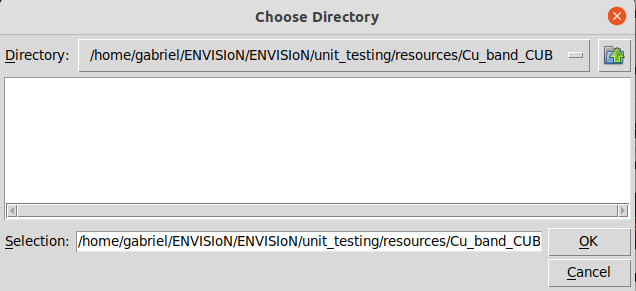
\includegraphics[scale = 0.56]{Images/newGUI_VASPdir.png}
    \caption{Standing inside a VASP-directory.}
    \label{fig:newGUI_VASPdir}
\end{figure}

\subsection{Parse Selected Folder}
When a folder has been loaded the contents need to be parsed into HDF5-format in order to enable visualization. The "Parse Selected Folder" button will use the appropriate parser to convert the contents of the files in the VASP-directory into a HDF5-file which is loaded into the dataset. After correctly loading and parsing a VASP-directory, the GUI should look as in figure \ref{fig:newGUI_parsedVASP}.

\begin{figure}[H]
    \centering
    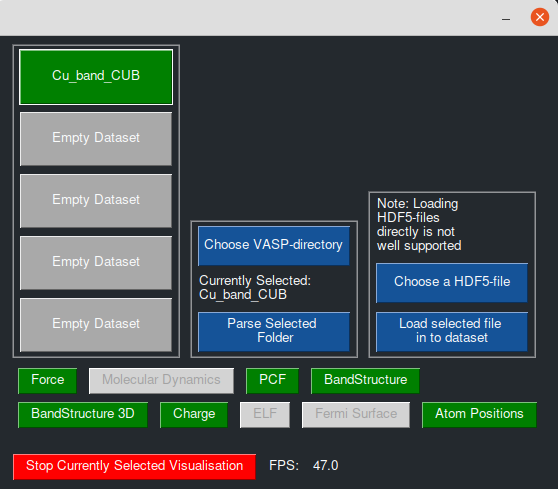
\includegraphics[scale = 0.56]{Images/newGUI_parsedVASPdir.png}
    \caption{How the GUI looks after the user has loaded and parsed a VASP-directory.}
    \label{fig:newGUI_parsedVASP}
\end{figure}

\subsubsection{Choose a HDF5 file}
If instead of selecting a VASP-directory and parsing the contents into HDF5-format the user may load an already parsed HDF5-file by pressing the "Choose a HDF5-file" button. This essentially means that the parsing step is skipped since in the "Choose VASP-directory" option the contents of the VASP-directory is parsed into the HDF5-format and then loaded into a dataset. In this option the HDF5-file, which may have been produced by parsing a VASP-directory or a similar format, is directly loaded into the desired dataset. 

\subsection{Active datasets}
When a dataset is loaded for visualisation its name will be visible in the selected dataset box, as seen in figure \ref{fig:newGUI_parsedVASP}. 

\subsubsection{Starting the visualisation}
By clicking on one of the active datasets under ``Active datasets'', the possible visualizations will be represented as green buttons, see figure \ref{fig:newGUI_parsedVASP}. The user can then choose what to visualize, by pressing one of the buttons. 

\subsubsection{Visualization controls}
After choosing a visualization, the user can change the properties of the current visualization. This may include changing the radius of the atoms in the visualization, altering the opacity of the atoms, switch between showing and hiding force vectors or many other options depending on what data was initially selected for the visualization. \newline \newline
The controls which are available for all different types of visualization, except for PCF, Bandstructure, Bandstructure 3D and Atom Postions, are:
\begin{itemize}
  \item Set atom radius
  \item Set opacity
  \item Toggle Canvas
\end{itemize}

The control available for the force-visualization is:
\begin{itemize}
  \item Toggle Force Vectors
\end{itemize}

The different controls for the molecular dynamics visualization (which are also shown in figure \ref{fig:newGUI_moldynSettings} and \ref{fig:newGUI_moldynSettingsChanged}) are:
\begin{itemize}
  \item Play/Pause, which stops or starts the animation
  \item Set animation speed
\end{itemize}

\begin{figure}[H]
    \centering
    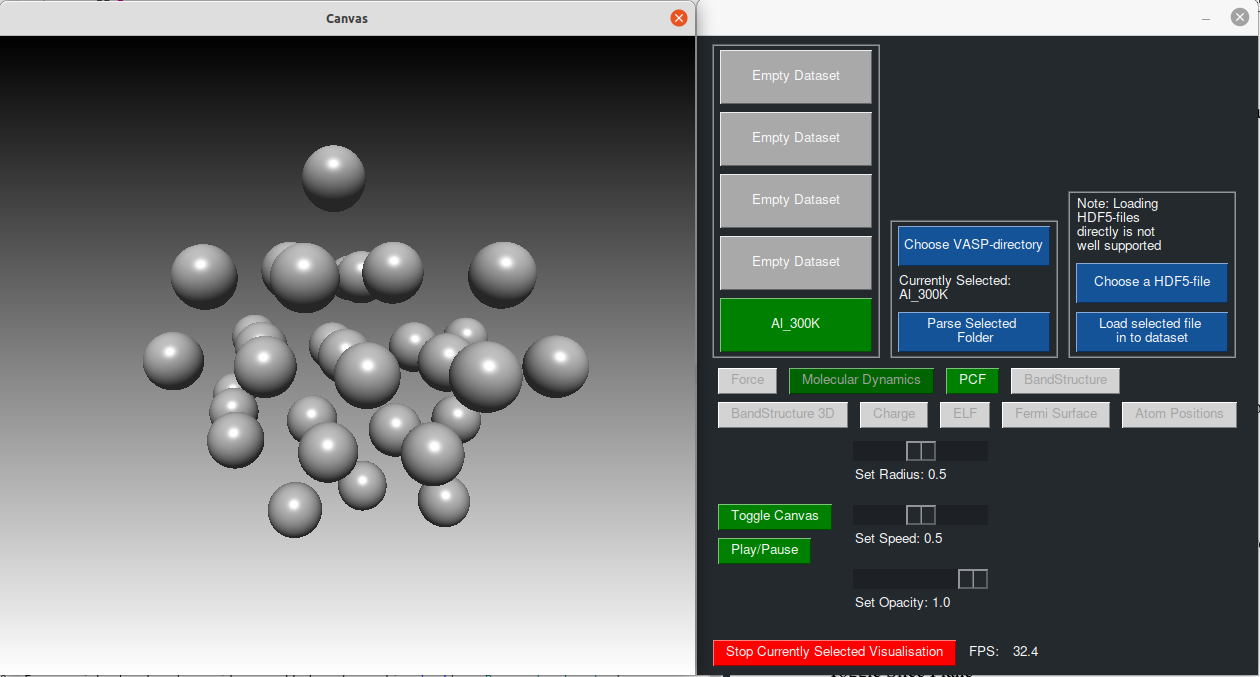
\includegraphics[scale = 0.40]{Images/newGUI_moldynSettings.png}
    \caption{Demonstration of the visualization controls available for molecular dynamics.}
    \label{fig:newGUI_moldynSettings}
\end{figure}

\begin{figure}[H]
    \centering
    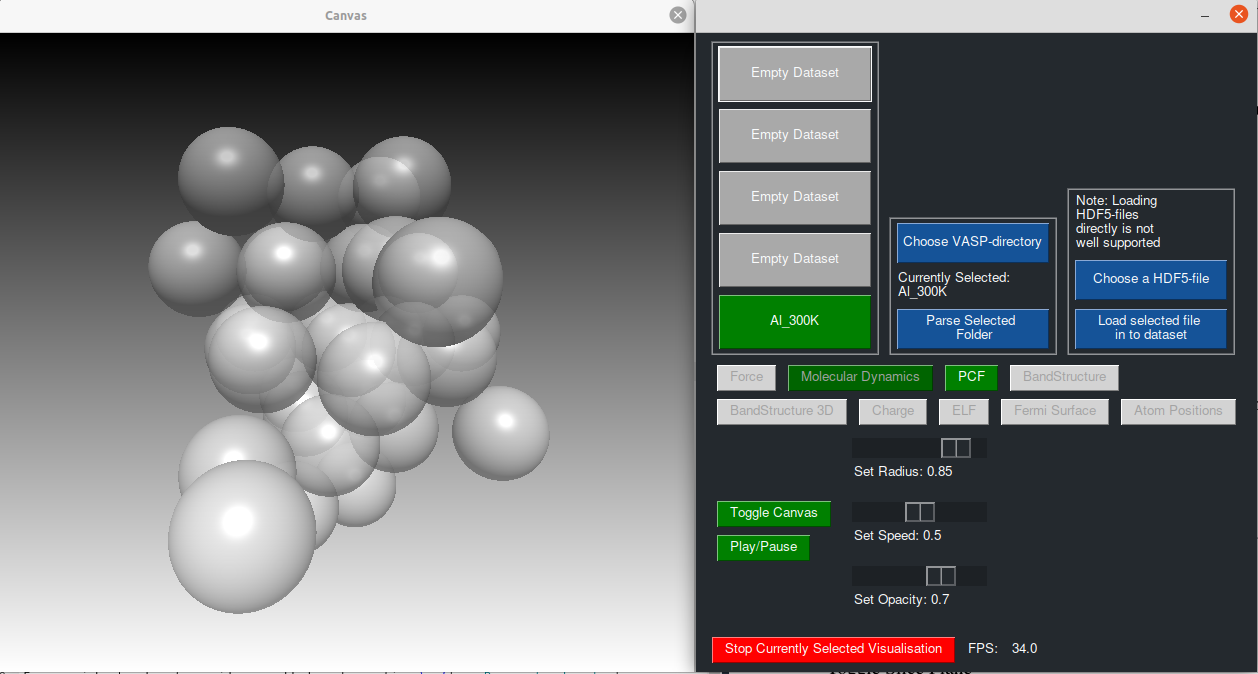
\includegraphics[scale = 0.40]{Images/newGUI_moldynSettingsChanged.png}
    \caption{Molecular dynamics visualizations with some visualization-properties changed.}
    \label{fig:newGUI_moldynSettingsChanged}
\end{figure}

The different controls for the charge and ELF visualization are:
\begin{itemize}
  \item Toggle ISO surface
  \item Toggle Slice Canvas
  \item Toggle Slice Plane
  \item ISO Surface Value
  \item Slice Plane Height
  \item Shading Mode
  \item Volume Selection
\end{itemize}

The different controls for the ELF visualization is:
\begin{itemize}
  \item Toggle ISO surface
  \item Toggle Slice Canvas
  \item Toggle Slice Plane
  \item ISO Surface Value
  \item Slice Plane Height
  \item Shading Mode
  \item Volume Selection
\end{itemize}

\subsection{If ENVISIoN does not respond or crashes}
There are three ways in which a crash may occur during the operation of the GUI. The first one involves Inviwo receiving a core dump error and terminating the current process. Why this happens is very difficult to decide and the reasons can sometimes appear arbitrary, restarting the GUI and trying again is recommended.

Another potential pitfall is errors occurring while reading from or writing an HDF5-file. The GUI is equipped with functions that make sure parsing produces a new HDF5-file whenever you load or overload a dataset. Should there be an issue with this you can start the GUI again and then press the exit button in the top right corner. This will delete all HDF5-files in the GUI directory and should prevent the same issue from occurring again. In the unlikely event that you are trying to directly load an HDF5-file that has the exact same name as one in an already loaded dataset the program will crash as well. This is because the HDF5-files need to be uniquely named.

The third risk of crashing is if something with the GUI-code would get stuck or crash. So far no instances of this has been recorded but there is obviously a risk that some combination of usage might produce such an error. 